%!TEX root = ../main.tex

 In terms of scope the aim of the method is to produce plausible lighting for Augmented Reality applications, and thus increase the sense of realism of the composed graphics. This does not mean that imagery that would for all practical purposes be indistinguishable from reality will be achieved. As said earlier, the incompatible lighting is only one of the problems with current AR graphics. In order to achieve complete realism all the other problems would have to be tackled as well. The method also does not attempt to improve other aspects of AR, such as tracking. And so the experiment is designed only to evaluate the similarity of a real object and a virtual representation of the same object in the same controlled lighting conditions.\newline
\section{Setup}
In order to test the results a real object with a variety of materials was chosen, in this case it was an Xbox 360 controller with a custom paint job. A 3D model of the same Xbox 360 controller was modified to match the custom paint job and the materials were replicated as closely as posible to the real object using Unity's built-in shaders. In the end 4 main shaders were used, a highly reflective plastic for the borders and some of the buttons, a more matte plastic for the main body, a completely specular chrome for the Xbox button and a semi-transparent and glossy plastic for the colored buttons. The choice of this motif was based both on the ease to find a reliable 3D counterpart for a real object and on the already wide variety of materials present in the object.\newline
In order to provide a ground truth for a reliable size by side comparison a screen capture of the application running while both the real and virtual object are in the frame, in similar positions and orientations and affected by controlled lighting that is also simulated using the method for the virtual counterpart. Another experiment will be a direct substitution, leave the controller on the table, remove it from frame and place the marker instead, in a way such that the virtual controller will appear in a similar position and orientation in order to provide a clear comparison, everything remains the same and both objects can be appreciated in the exact same setting.\newline
As for benchmarking how this method stands in comparison to other similar ones, the conditions of the experiments presented in the results section for the methods in \cite{kanbara2004}, \cite{karsh2014} and \cite{pessoa2011} are replicated in terms of similar setting and virtual objects used. The resulting images are compared to the ones from their methods. In order to replicate these settings additional 3D models are needed, namely a teapot and the dragon and Buddha from the Stanford 3D Scanning Repository.\newline
The actual way in which the experiment is conducted is defined in the following scenario:
\begin{itemize}
    \item \textbf{Setting:} A room with consistent and invariable lighting is used and some kind of flat, matte surface to lay the objects on. An Xbox 360 controller with the characteristics described previously and a marker to track the virtual object.
    \item \textbf{Requirements:} A mobile device running the developed demo application, a marker for virtual objects. A real object and its corresponding virtual counterpart, modelled as close as possible. Common 3D models from the Stanford 3D Scanning Repository.
    \item \textbf{Goals:} Obtaining a set of images that will enable readers and experimenters alike to make a fair comparison of the method application, side by side with a real object counterpart.
    \item \textbf{Actions:} Place the controller on the surface, and capture and image. Then remove the real controller and substitute it with the marker in a way that the virtual controller appears in the most similar position and orientation possible; capture an image in the end as well. Replicate the scenarios in \cite{kanbara2004}, \cite{karsh2014} and \cite{pessoa2011} using teapots, Buddahs and dragons and capture images of each.
     \item \textbf{Benchmark:} The image result yielded by the method, as well as the time per frame will be captured and used for comparison's sake and benchmarking head to head with the results from similar methods.
\end{itemize}

It's important to also mention the need of replicating the previous work's settings and the reason why. In some cases the product is not a runtime application, and thus the only applicable comparison is image-based. The authors of other runtime methods were approached to evaluate the possibility of using their binaries to produce images and they either declined or gave no answer. And so the only possible comparison is image to image and taking their word for the performance indications in the form of frames per second.\newline

\section{Results}

\underline{Experiment 1: Game controller: } This experiment produced quite satisfactory results, the materials and the position and orientation on the virtual object are not exactly the same, and so the highlights shining off the surface are not in the same places. But the shadow shows that the light is placed in a very acceptable approximation of the real light. The application is running at 24 FPS on this screen capture and it's a good measure of the average of performance. 
\begin{figure}[H]
    \centering
    \begin{minipage}{0.5\textwidth}
        \centering
        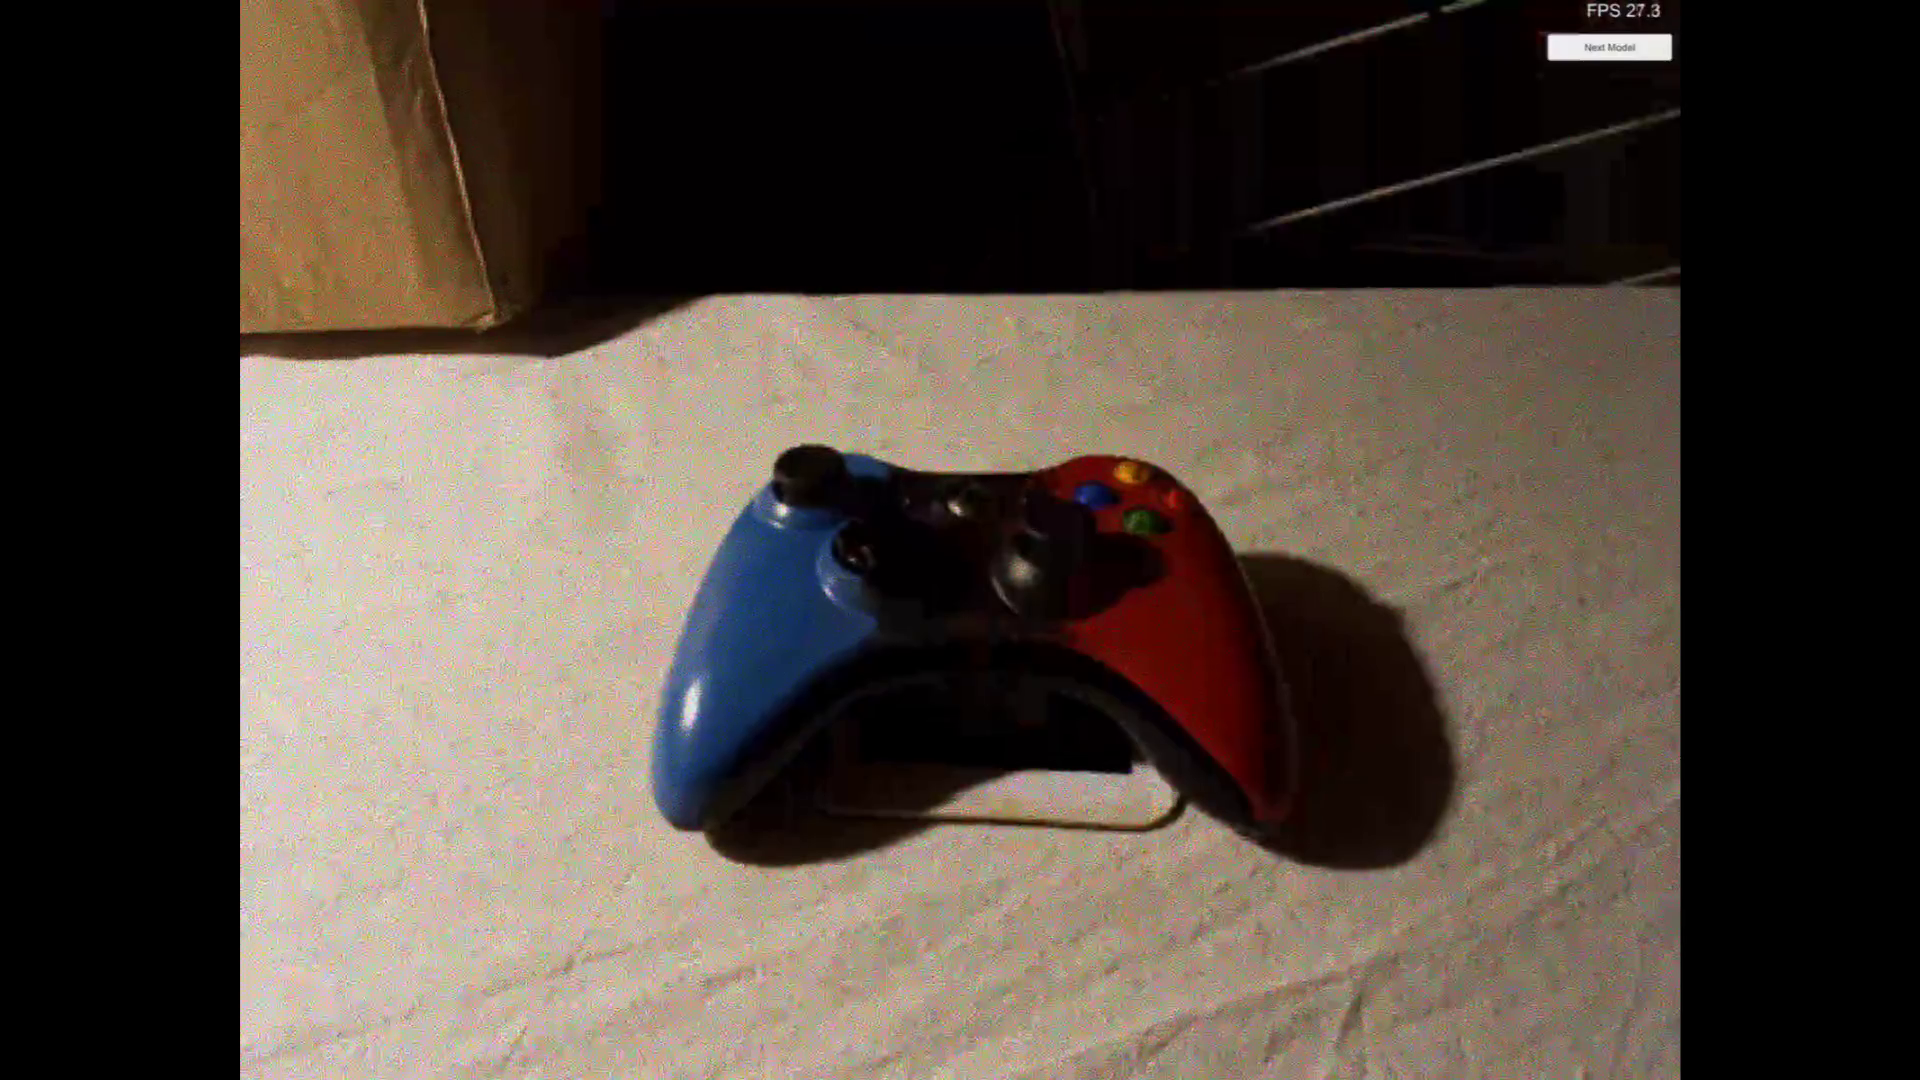
\includegraphics[width=0.99\textwidth]{Figures/ContReal.png} % first figure itself
        \caption{Real object: Custom painted Xbox 360 controller}
    \end{minipage}\hfill
    \begin{minipage}{0.5\textwidth}
        \centering
        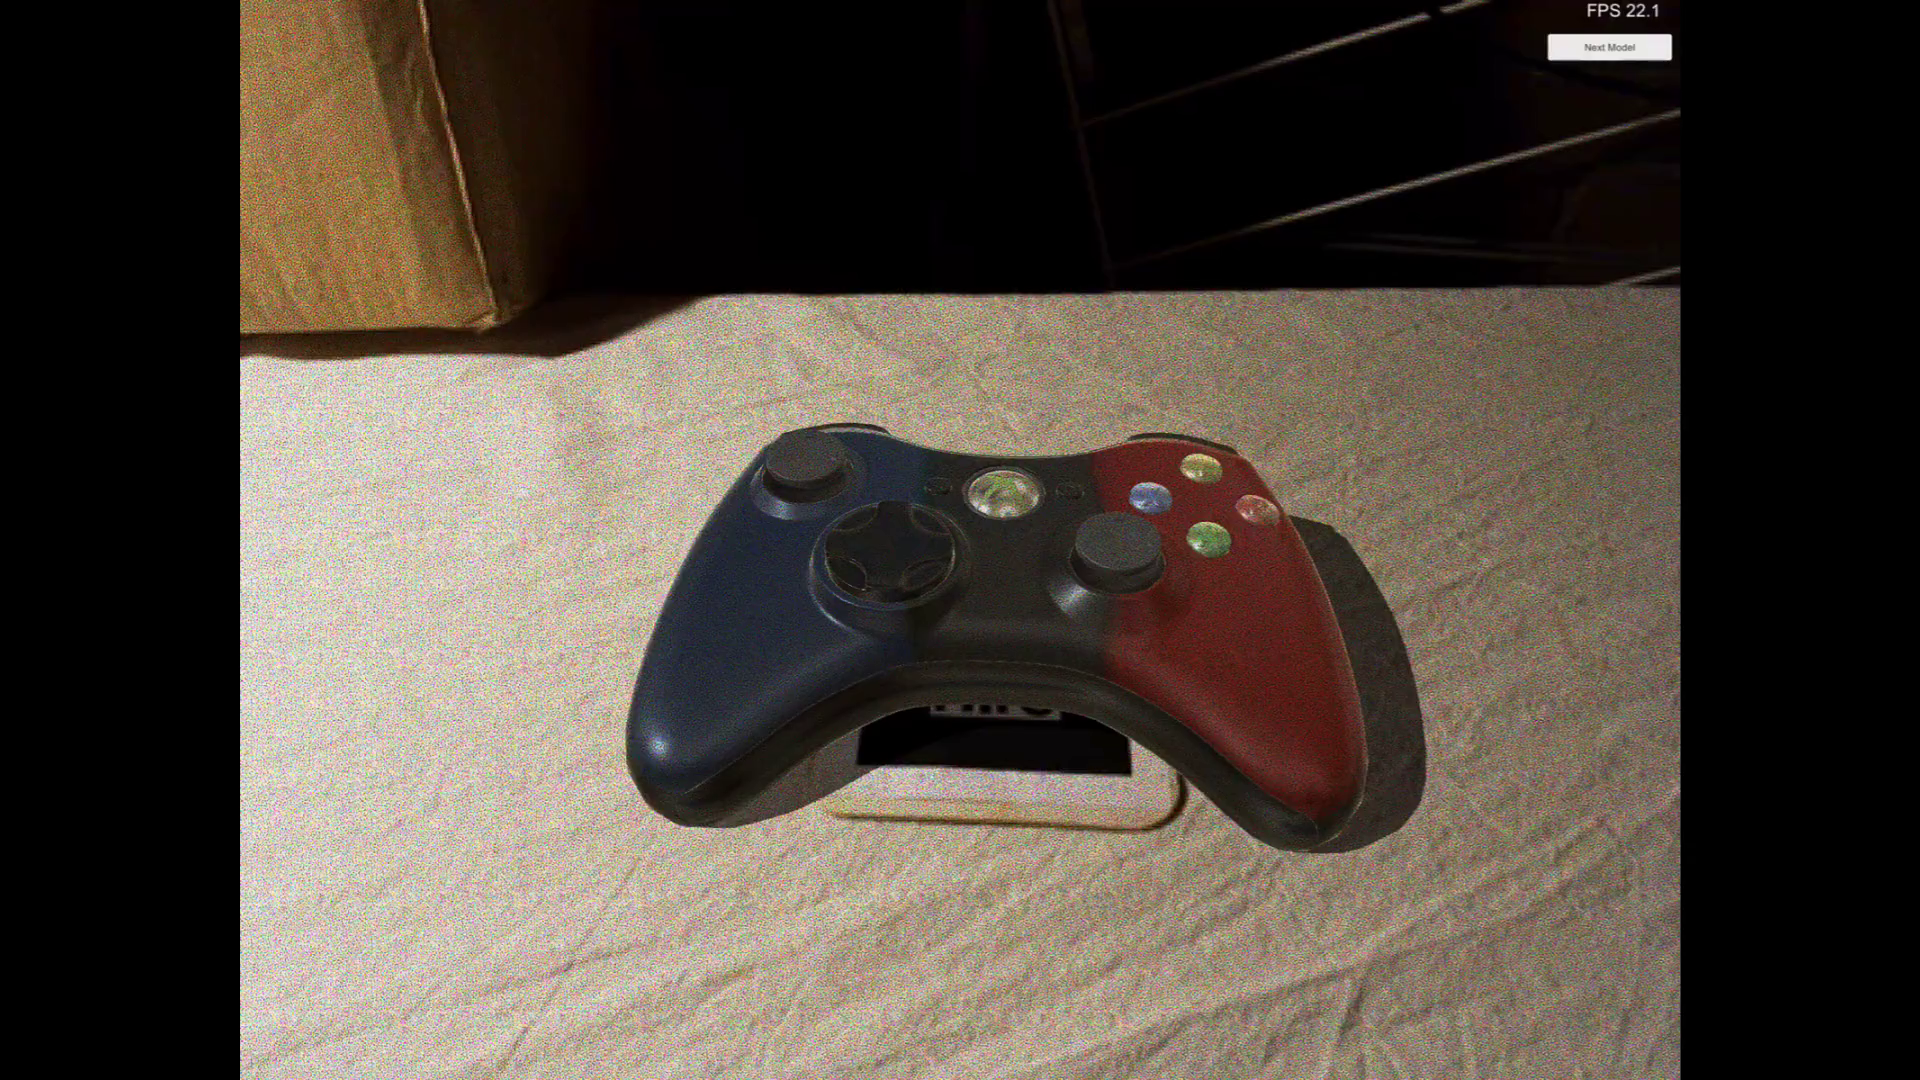
\includegraphics[width=0.99\textwidth]{Figures/ContVirtual.png} % second figure itself
        \caption{Virtual counterpart of the same object}
    \end{minipage}
\end{figure}

\underline{Experiment 2: Karsch's scenario: } This scenario was hard to replicate, due to the unusual framing and placing of the objects. The image produced by this method is plenty different, and the method it's being compared with is not a runtime method, but even so there are conclusions that can be drawn. In the image produced by Karsch's application it's hard to say if the lighting in the real and virtual parts of the image really correspond, the light sources, except for one, are not present in the frame and there are no similar real objects to the virtual ones that would serve as ground truth. In this methods result there is enough evidence to prove that the lighting in both the real and virtual worlds is similar, with cues such as the presence of real objects and their shadow directions.\newline
In this methods application the framerate at 21 FPS is still quite acceptable considering that there are 6 virtual dense models, but given the fact that Karsch's method is not interactive there's no possibility to compare in this regard.
\begin{figure}[H]
    \centering
    \begin{minipage}{0.5\textwidth}
        \centering
        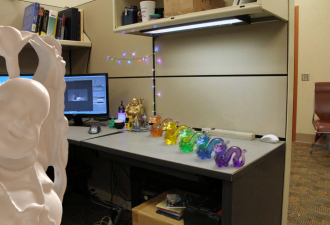
\includegraphics[width=0.99\textwidth]{Figures/budaDragonKarsch.png} % first figure itself
        \caption{Karsch's method results}
    \end{minipage}\hfill
    \begin{minipage}{0.5\textwidth}
        \centering
        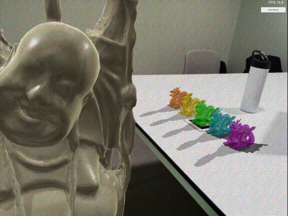
\includegraphics[width=0.99\textwidth]{Figures/budaDragon.png} % second figure itself
        \caption{This methods's results}
    \end{minipage}
\end{figure}


\underline{Experiment 3: Kanbara and Pessoa's scenarios: } These two scenarios will be grouped together due to the fact that the steps to replicate the experiment are the same. They both presented ceramic material teapots with a lighting setting that they did not specify. 
\begin{figure}[H]
    \centering
    \begin{minipage}{0.5\textwidth}
        \centering
        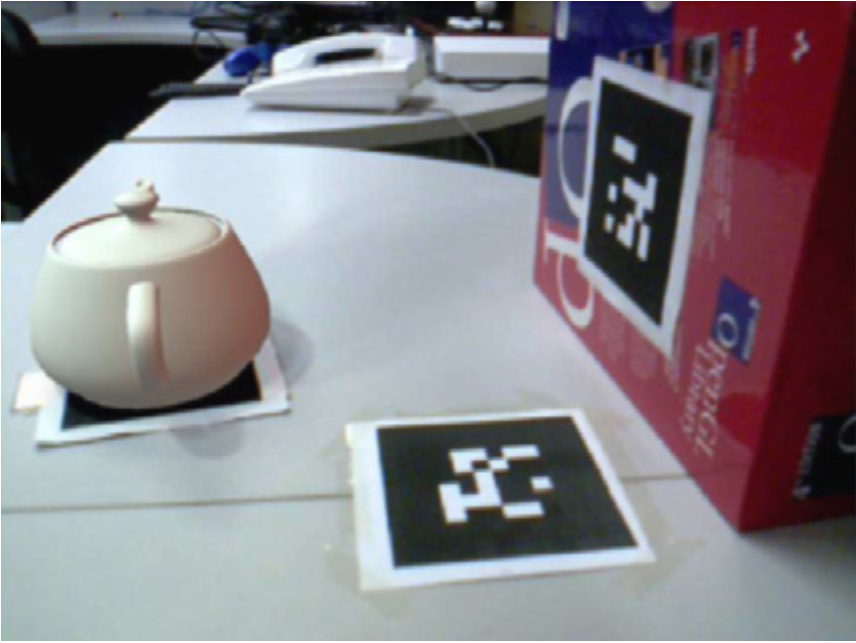
\includegraphics[width=0.99\textwidth]{Figures/Pessoa.png} % first figure itself
        \caption{Pessoa's method results}
    \end{minipage}\hfill
    \begin{minipage}{0.5\textwidth}
        \centering
        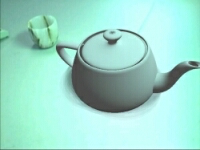
\includegraphics[width=0.99\textwidth]{Figures/kanbara.png} % first figure itself
        \caption{Kanbara's method results}
    \end{minipage}\hfill
\end{figure}

Both results look well blended into the environment, however in Pessoa's case it also must be said that the lighting setting is not disclosed and is not obvious from just looking at the results. For the aforementioned method there's also a considerable amount of pre-production required for the method to actually work, and the performance has a rather bad scaling, ranging from 180 fps with no objects to 5 fps with seven objects. The method in this work doesn't have those problems, the only pre-step required is to take a spherical panoramic image with the same device and no technical knowledge necessary;  and performance scales better going from 24 fps with a single object to 21 with six.\newline
In the case of Kanbara's results they look really good, the downsides to their method that the one here resolves are the need for a physical 3D marker to probe lighting and the performance, they report 20 FPS on a computer for the experiment they published. It's admittedly a 10 year old computer at the time of this writing, but the method proposed here is achieving slightly better framerates on a mobile device.\newline

\begin{figure}
  \centering
  \setlength{\unitlength}{\textwidth} 
    \begin{picture}(1,0.5)
       \put(-0.1,0){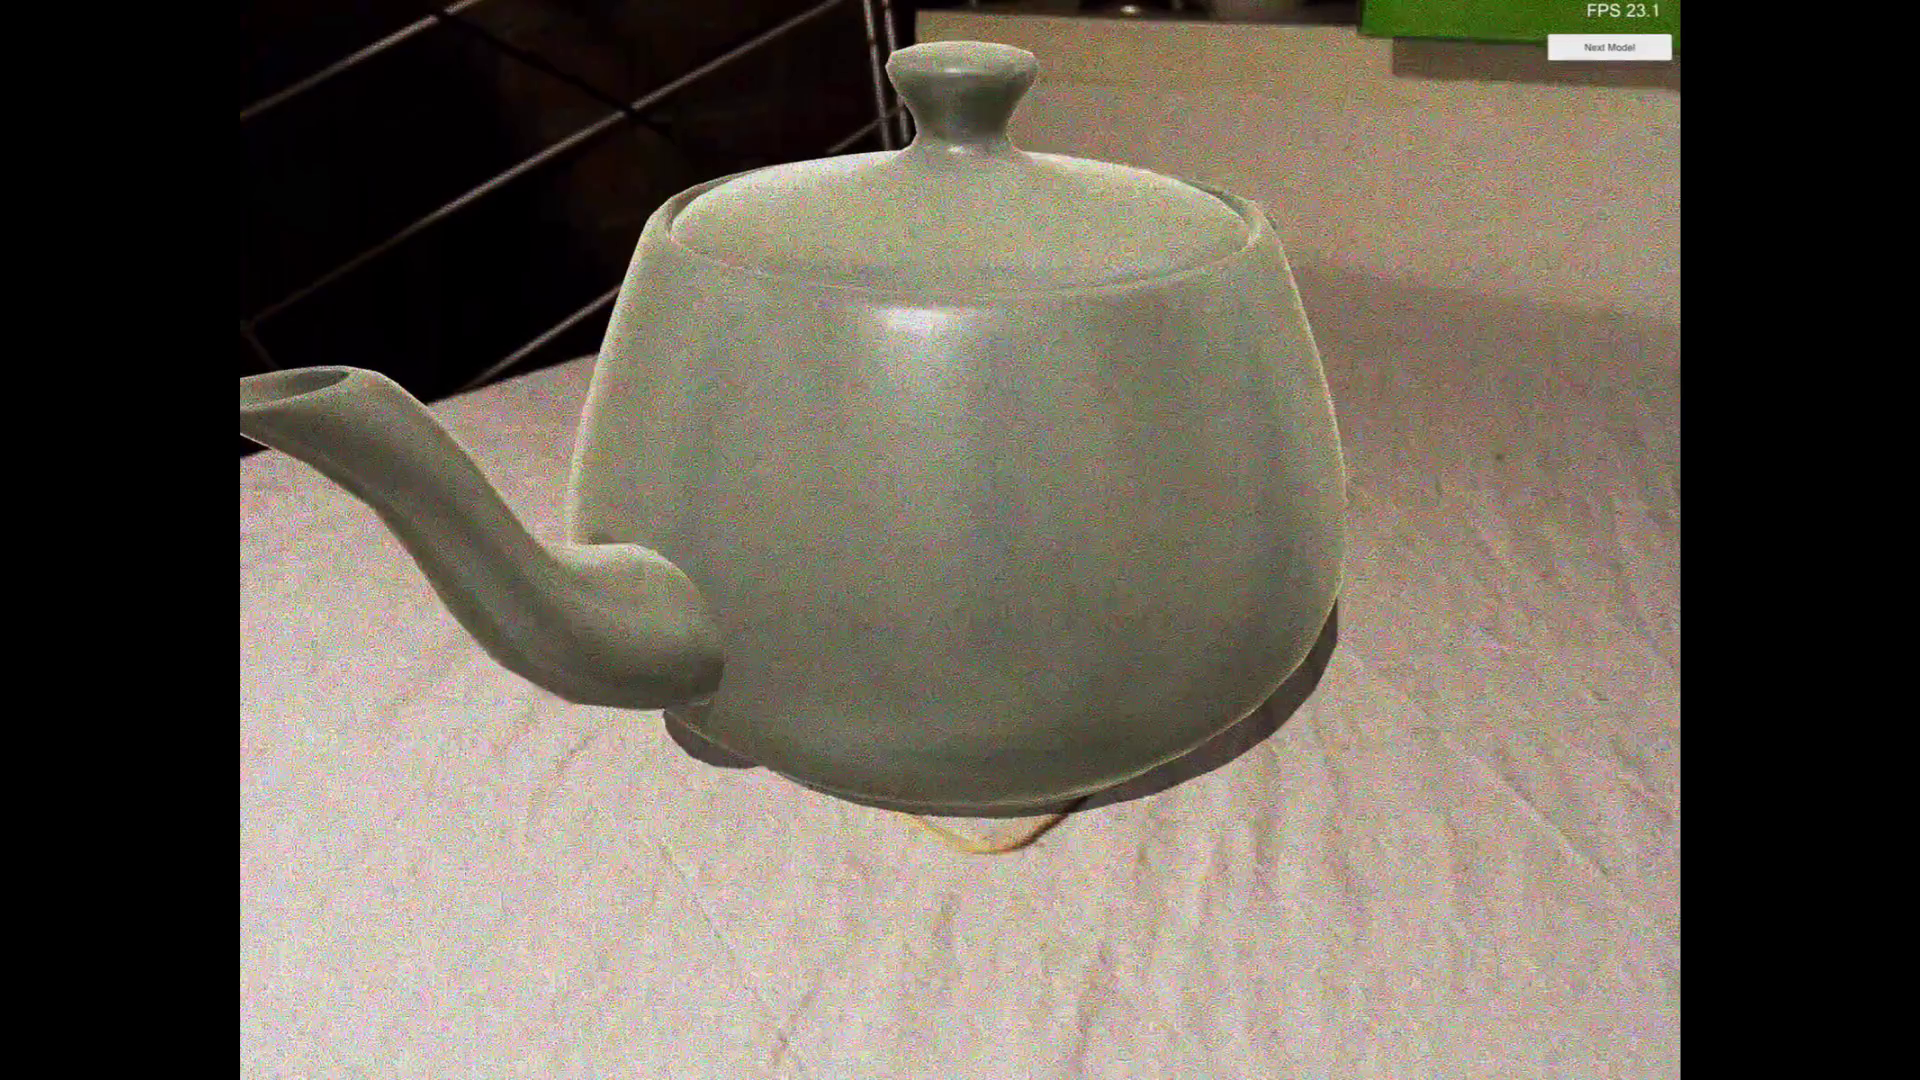
\includegraphics[width=0.99\unitlength]{Figures/kanbaraComp.png}}
       
    \end{picture}
    \caption{This method's teapot result}
\end{figure}

\section{Gallery}

Here are a few more screen captures from the application that show the potential of the method for the reader to draw their own conclusions.

\begin{figure}[H]
    \centering
    \begin{minipage}{0.5\textwidth}
        \centering
        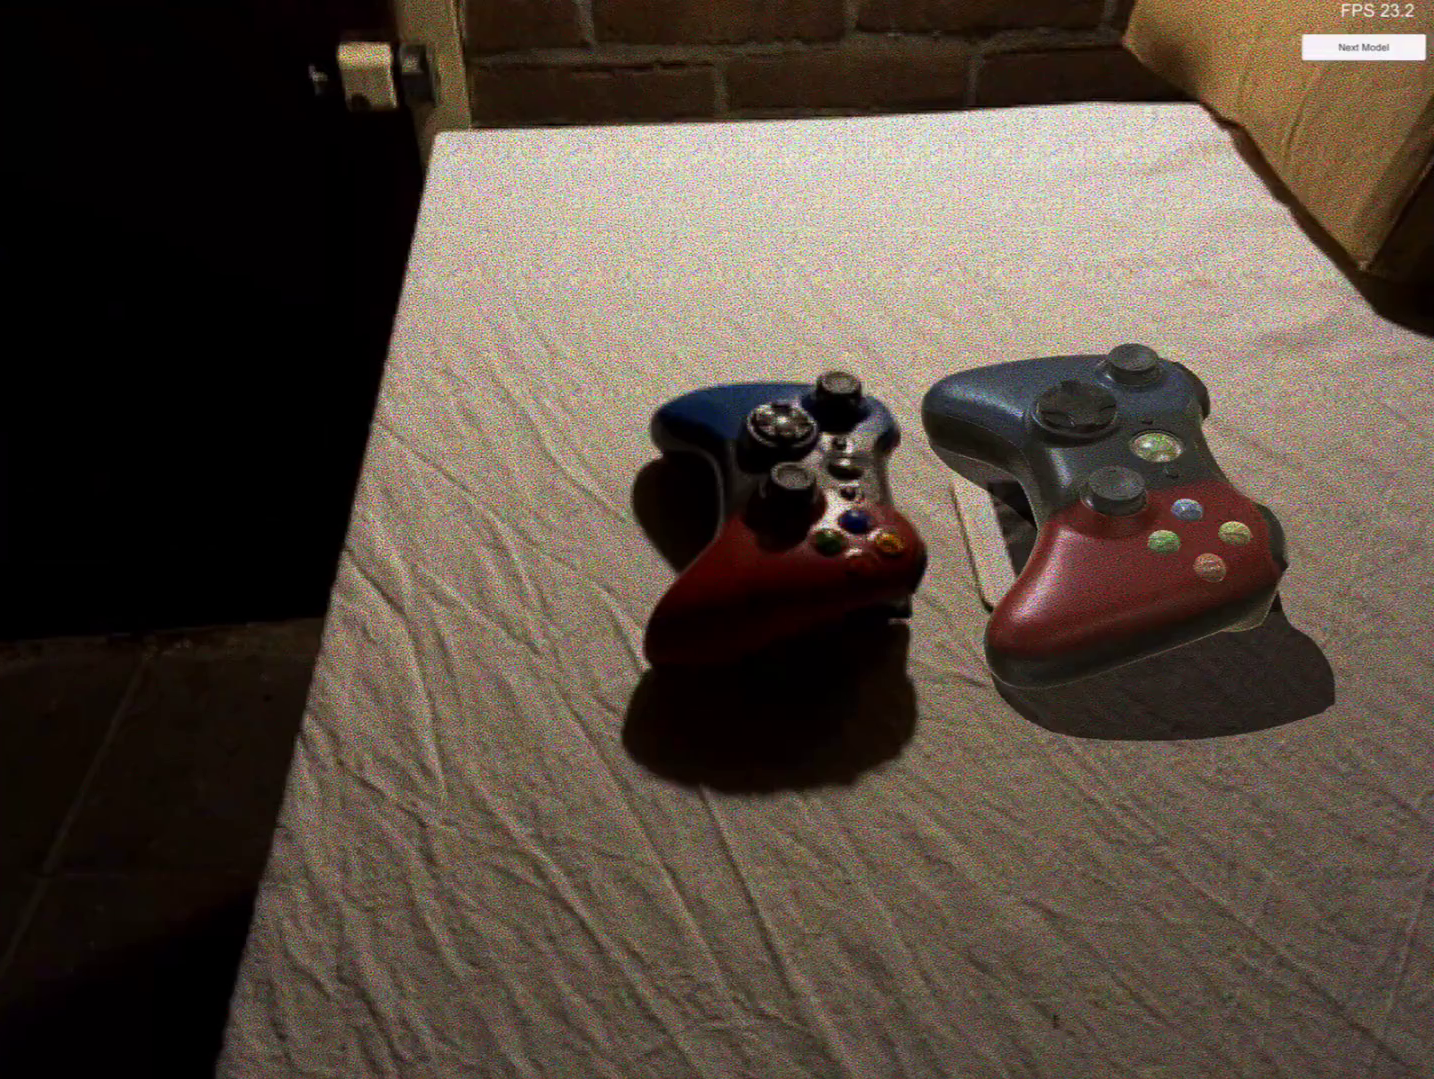
\includegraphics[width=0.99\textwidth]{Figures/ContBoth.png} % first figure itself
 
    \end{minipage}\hfill
    \begin{minipage}{0.5\textwidth}
        \centering
        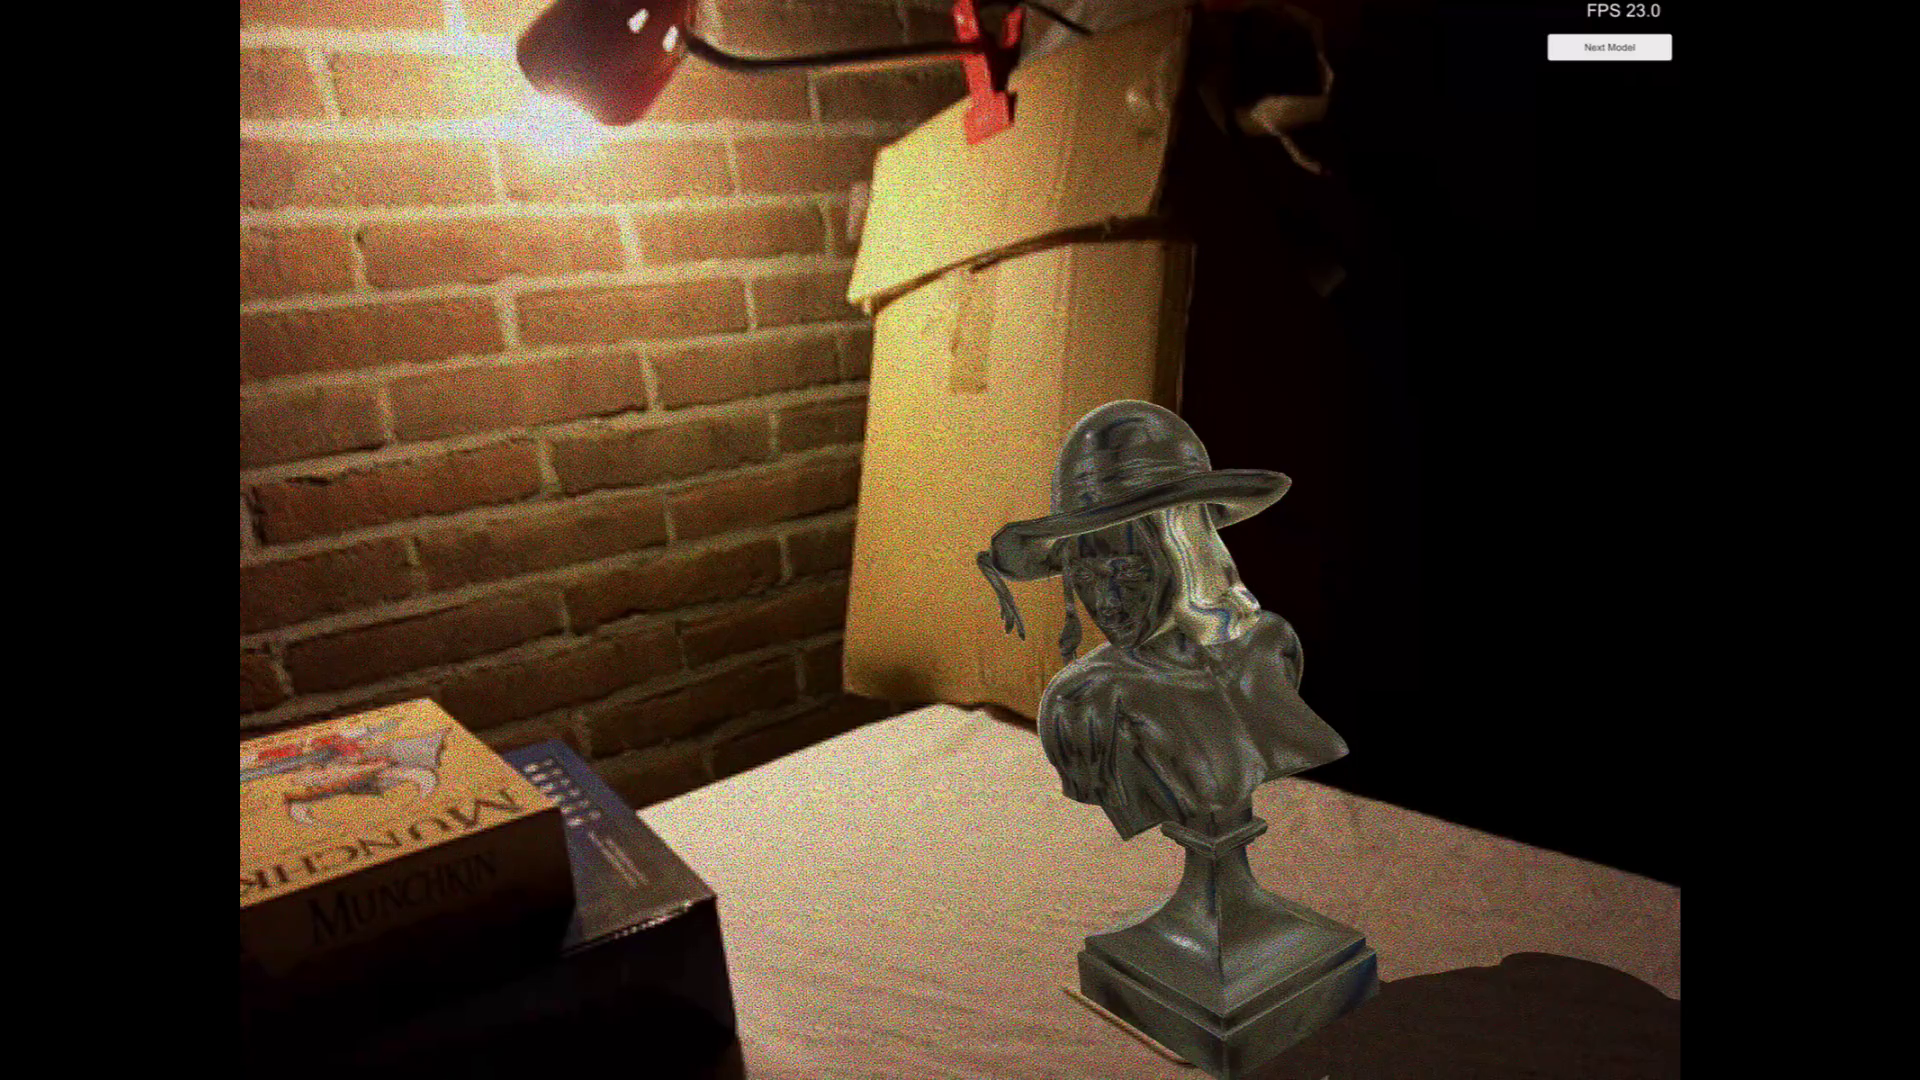
\includegraphics[width=0.99\textwidth]{Figures/Lena1.png} % second figure itself
    \end{minipage}\hfill
        \begin{minipage}{0.5\textwidth}
        \centering
        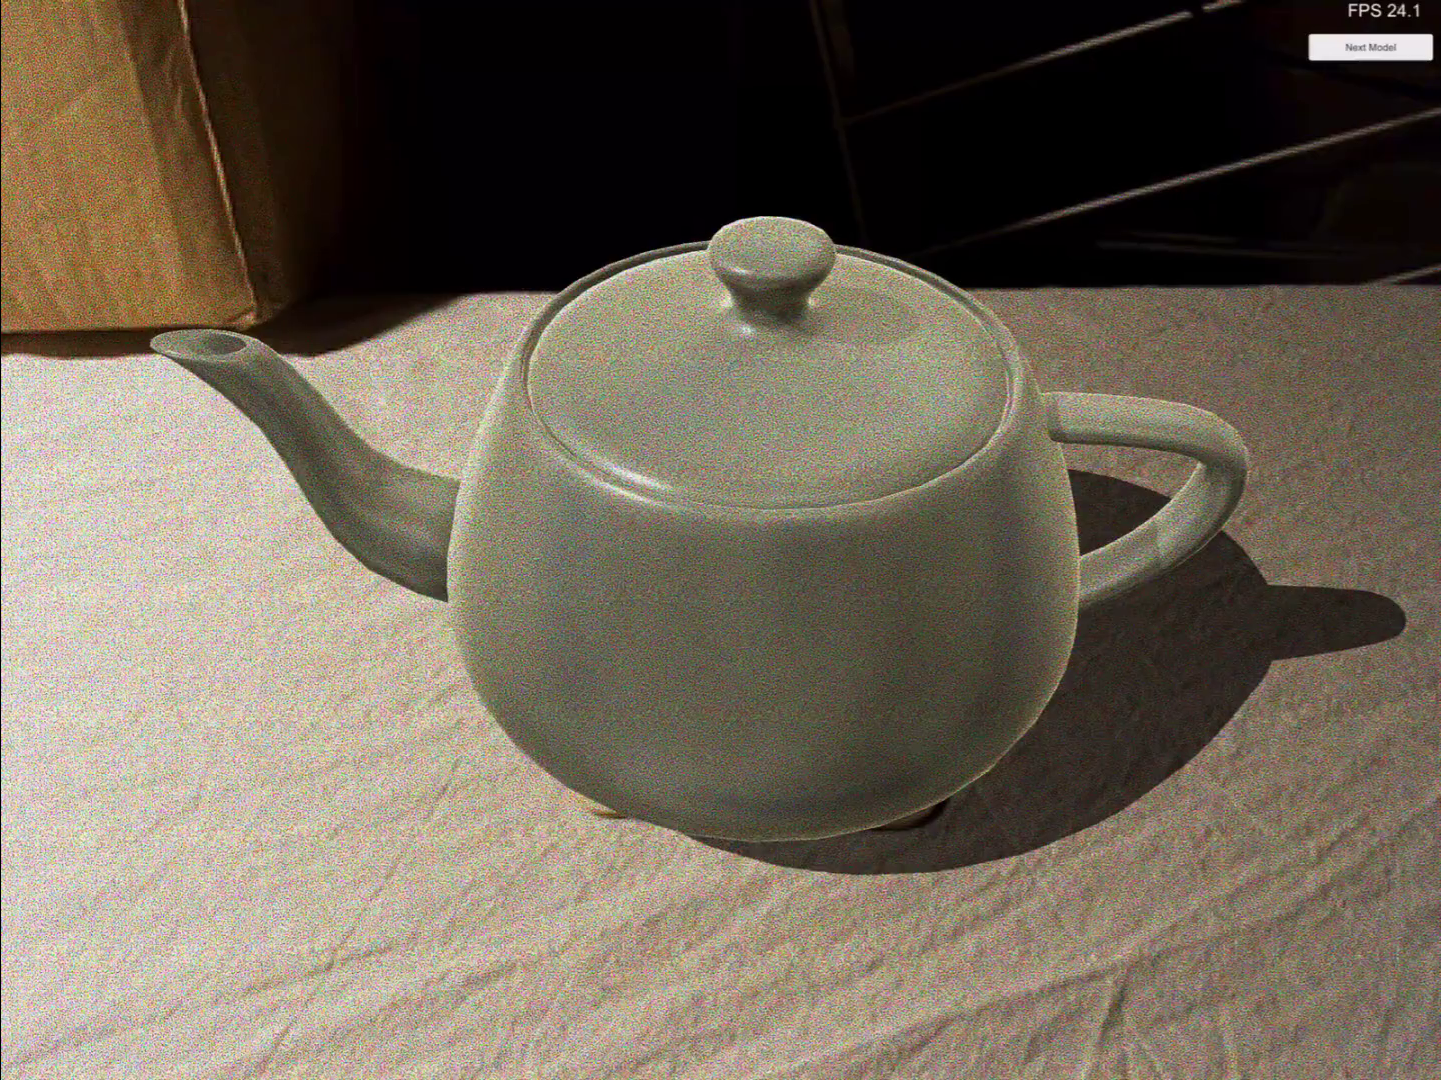
\includegraphics[width=0.99\textwidth]{Figures/TeapotVirtual.png} % second figure itself
    \end{minipage}\hfill
    \begin{minipage}{0.5\textwidth}
        \centering
        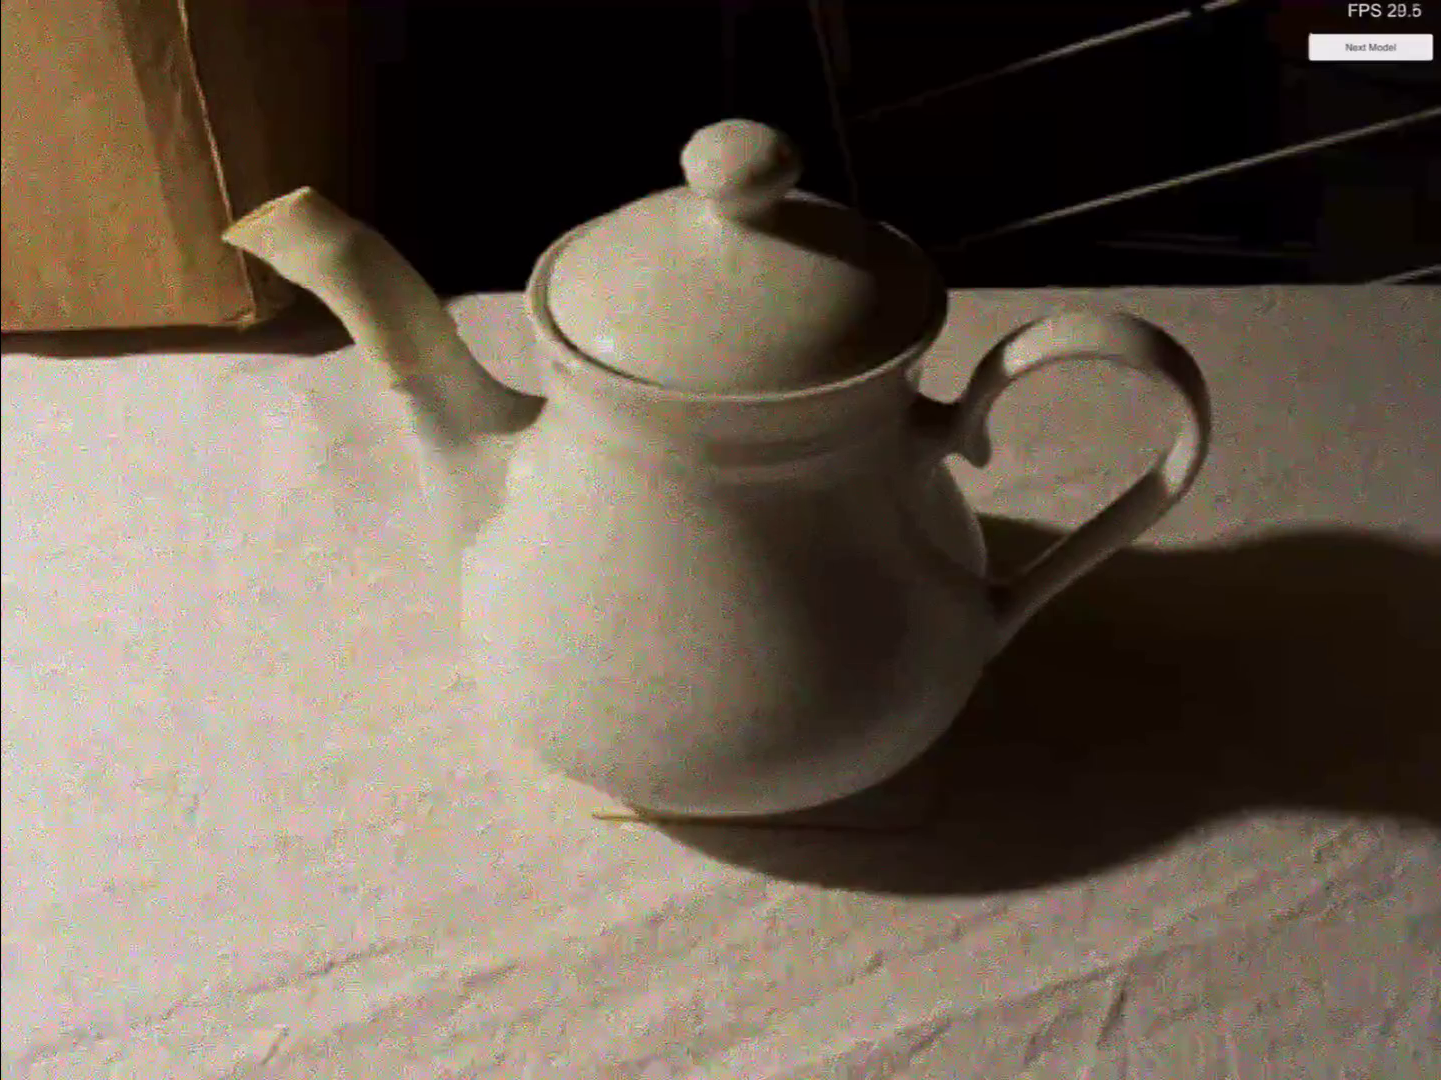
\includegraphics[width=0.99\textwidth]{Figures/TeapotReal.png} % first figure itself
    \end{minipage}
\end{figure}